\documentclass[11pt]{article}
\usepackage[utf8]{inputenc}
\usepackage[american]{babel}
\usepackage{parskip}
\usepackage{csquotes}
\usepackage{hyperref}
\usepackage{pdfpages}
\usepackage{times}
\usepackage[margin = 0.5in]{geometry}
\usepackage[natbib=true,
			citestyle=authoryear-comp, 
			hyperref=true,
			backend=biber,
			maxbibnames=99,
			uniquename=init,
			parentracker=true,
			giveninits=true, 
			uniquelist=false, 
			bibstyle=authoryear-comp, 
			maxcitenames=2,
    		url=false,
			]{biblatex}
\addbibresource{Remote.bib}
\usepackage{doi}
\DeclareLanguageMapping{american}{american-apa}


\begin{document}
% frontmatter
\title{A proposal towards proposed research in computational biology}
\date{06 November 2017}
\author{Graham Voysey (gvoysey@bu.edu),
	    Kat Elkind (kelkind@bu.edu),\\
	    Rachel Petherbridge (rpether@bu.edu),
	    Kestutis Subacius (kestas@bu.edu)}
\maketitle
% main text
\section{Specific Aims}
% 1 paragraph summary of the background of the project, the key problem or question, and a statement of the overall goals of the project.
Chimeric Antigen Receptor (CAR) T cell therapy engineers a cancer patient's T cells to express one or more synthetic antibodies chosen to specifically target that patient's cancer. This approach has shown remarkable success with acute lymphoblastic leukemia (ALL) when targeting CD19.  Recent work by \citet{Perna2017Integrating} sought to identify potential CAR targets for Acute Myeloid Leukemia (AML), with the goal of approaching the performance of ALL results.  While they identified no single target which was as promising as CD19, they identified a strategy by which paired weaker targets may be selected to maximize selectivity,  and offers several paired targets of interest.  The Wong Lab at Boston University seeks to extend this work by identifying more complicated combinatorial pairings of co-expressed targets which preserve the specificity of the effects, but allow the use of more potent but otherwise less specific antigens.   In this work, we propose to design a target selection algorithm to select candidate sets of four targets to allow the use of higher AML-affinity candidates which were excluded by \citeauthor{Perna2017Integrating} for their off-target effects by coupling them with AML-specific co-expressed sites.

To this end, we propose the following Specific Aims:
% 2-3 paragraphs describing each specific aim of the project.  Aims should be highly focused.

\begin{enumerate}
	\item{Preparation of Data Sources}
		\begin{itemize}
			\item proteomics data: huge.
			\item transcriptomics data: even more huge.
		\end{itemize}
	\item{Target Selection Algorithm}
		\begin{itemize}
			\item 
		\end{itemize}
\end{enumerate}
\section{Project Description}

	\subsection{Significance}
% why is the proposal important? how will it advance the field? what is the key problem we adddress? why do we care? 1 page or less.
CAR really works against AML and it needs to work against other cancers.  So far it works best when there's a rockstar target like CD19; the most promising way this approach generalizes is if multiple targets can be combined.
% Using a method known as \emph{adoptive cell transfer}, T cells are removed from a patient, made to express a particular chosen set of antibodies thought to best target that patient's tumor, and then reintroduced to the body.  
	\subsection{Innovation}
% how is our approach new and unique? how does this project use and extend computational methods in a novel way
	\subsection{Research Strategy}
% what we do and how. background, approach for each aim in turn.  provide enough detail to evaluate liklihood of success.  think through potential problems and address them. include sections on dataset availabliltiy, special resources to be used, and a timeline.  Include a collaboration plan, roles of individual investigators, and specific coordination of activities to ensure group success.
		\subsubsection{Background}

		\subsubsection{Aim 1...n}

		\subsubsection{Resources}
		\begin{itemize}
			\item datasets with links 
			\item wong's grad student 
			\item graham has cluster access if we need to flip big data
			
		\end{itemize}

		\subsubsection{Timeline}

		\subsubsection{Collaboration Plan}
		\begin{itemize}
			\item graham and kestas code
			\item rachel and kat: bio
			\item we have a grad student in wong's lab who wants to help, who are they 
			\item 
		\end{itemize}
\printbibliography[heading=bibintoc]{}
\newpage
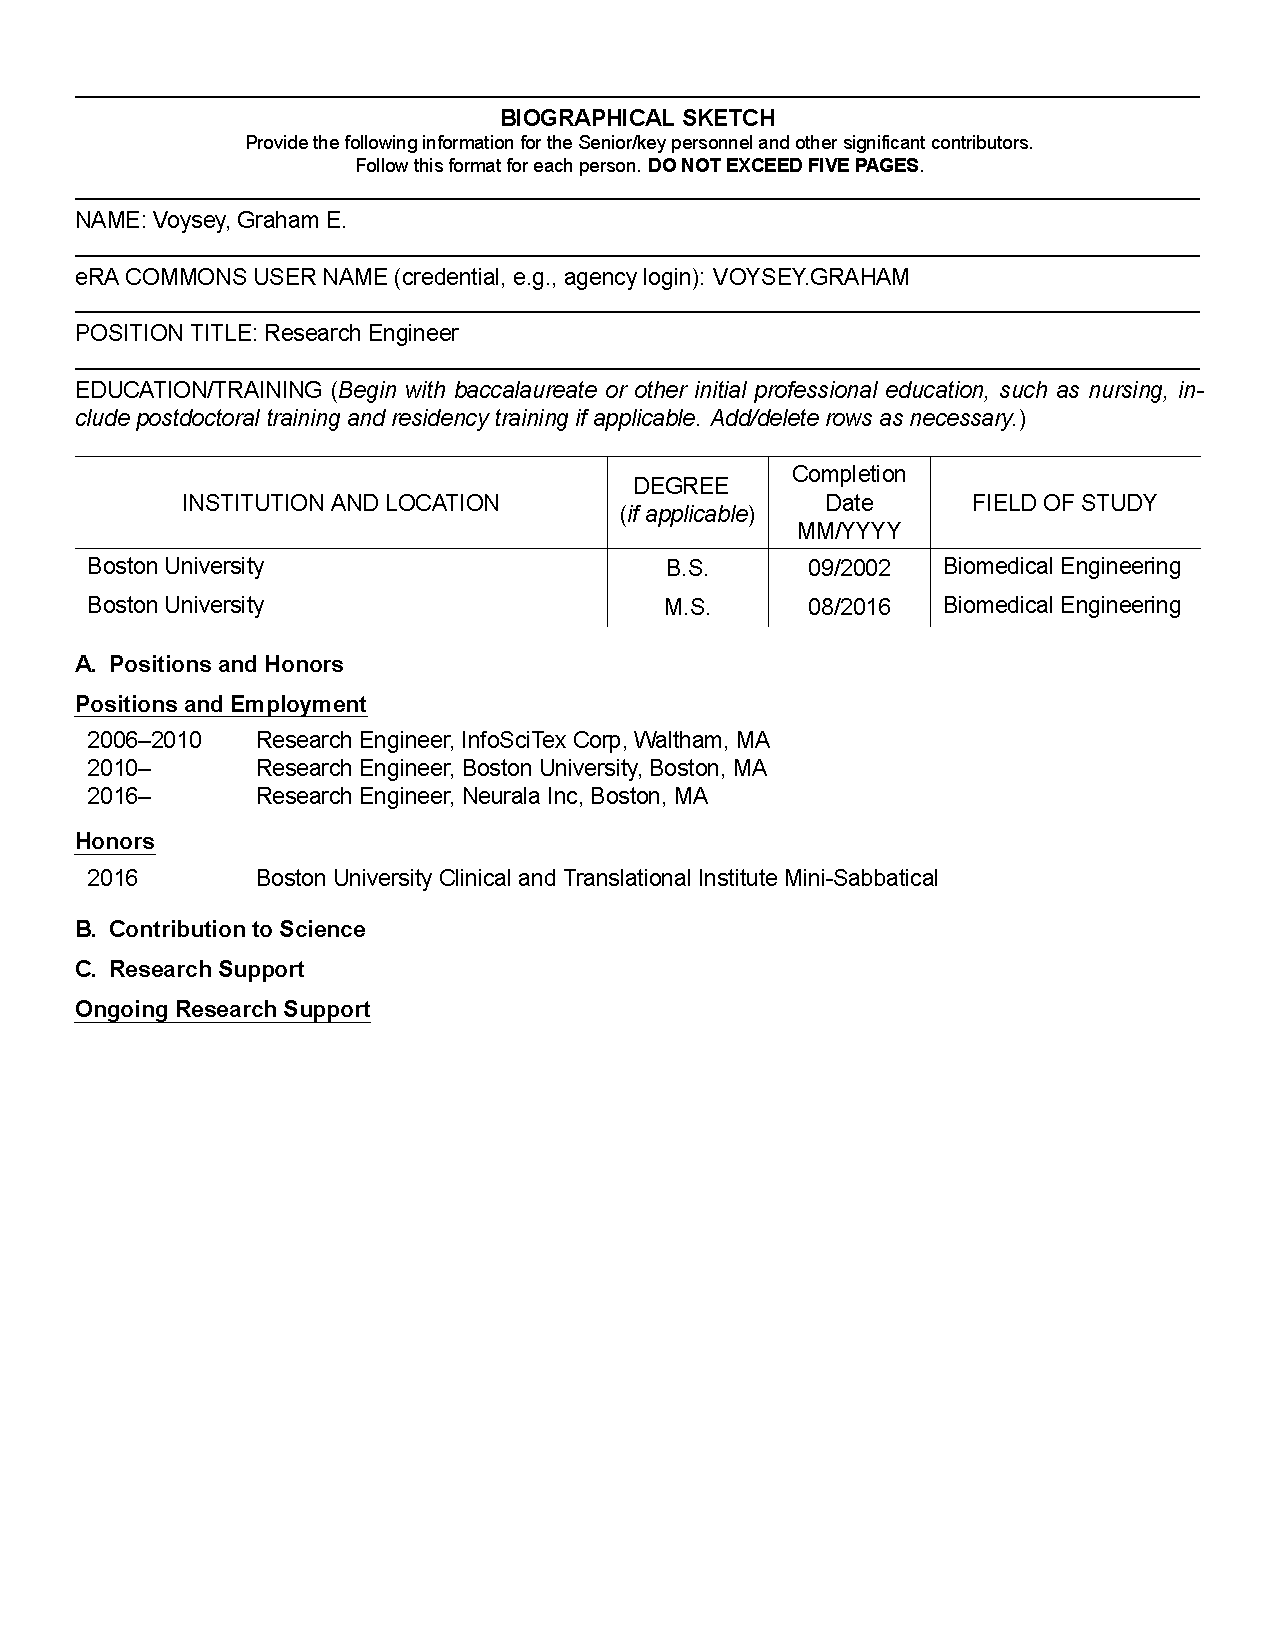
\includepdf{biosketches/gvoysey-biosketch.pdf}
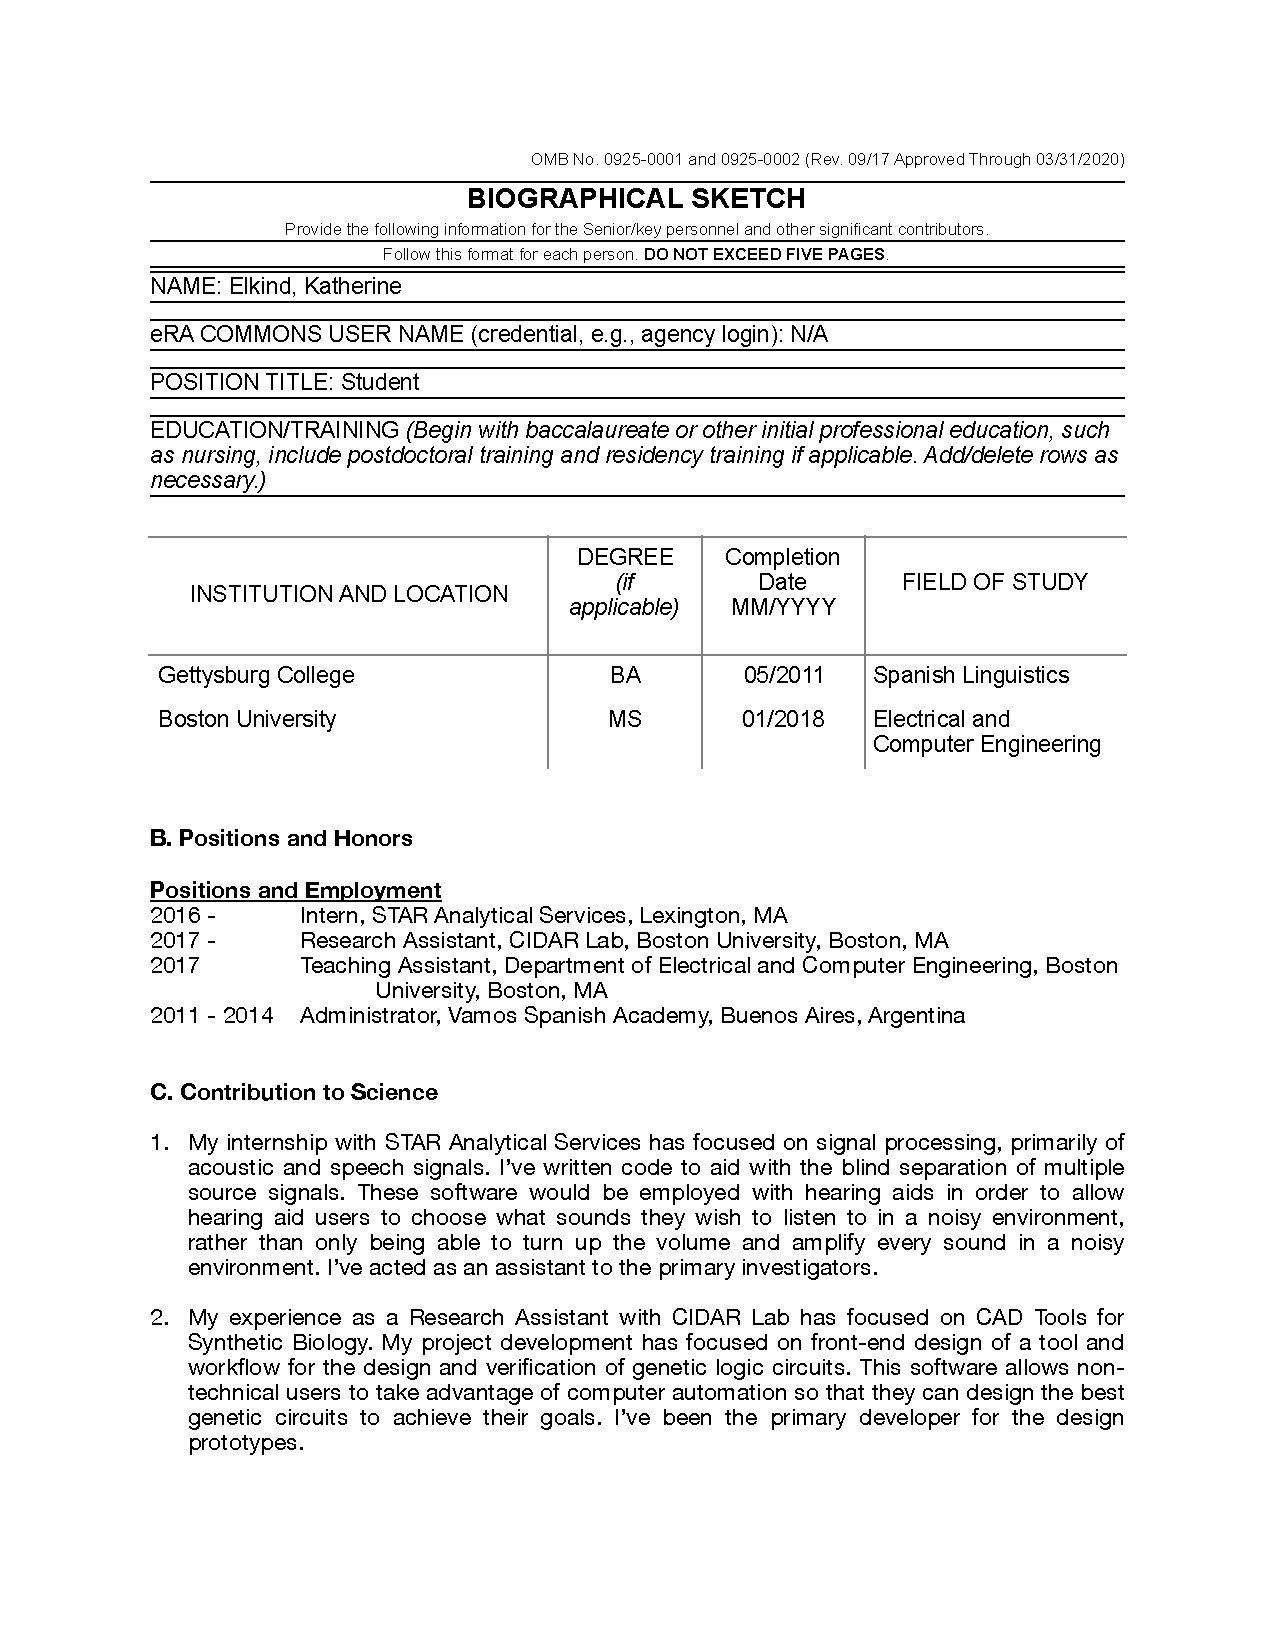
\includepdf{biosketches/Elkind_Katherine_Biosketch.pdf}
% \includepdf{biosketches/rpether-biosketch.pdf}
% \includepdf{biosketches/kestas-biosketch.pdf}

\end{document}